\documentclass[aps,pra,12pt,nofootinbib,superscriptaddress,longbibliography,showpacs]{revtex4-1}

\usepackage[utf8]{inputenc}
\usepackage[T1]{fontenc}
\usepackage[english]{babel}  % english language

\usepackage{amssymb,amsmath,amsfonts,amsthm}
\usepackage{mathtools}
\usepackage{verbatim}
\usepackage{enumerate}
%\usepackage{tensor}
\usepackage{fancyhdr}
\pagestyle{fancy}
\usepackage{graphicx}
\graphicspath{{pics/}}
\usepackage{hyperref}
\usepackage{bbm}


\newcommand{\bydef}{\stackrel{\mathrm{def}}{=}}
\renewcommand{\baselinestretch}{1}  % cancels any possible double spacing

\usepackage{color}
%Some shortcuts added for edits
\definecolor{dred}{rgb}{.8,0.2,.2}
\definecolor{ddred}{rgb}{.8,0.5,.5}
\definecolor{dblue}{rgb}{.2,0.2,.8}
% suggested change
\newcommand{\add}[1]{\textcolor{dred}{*** #1 ***}}
% suggested to remove
\newcommand{\out}[1]{\textcolor{ddred}{\textbf{[}\emph{#1}\textbf{]}}}
% comment or remark
\newcommand{\yo}[1]{\textcolor{dblue}{\textbf{[}#1\textbf{]}}}
\newcommand{\todo}[1]{\textbf{\underline{\textcolor{dblue}{\textbf{[}#1\textbf{]}}}}}

\theoremstyle{plain}
\newtheorem{theorem}{Theorem}   %[section]
\newtheorem{proposition}[theorem]{Proposition}
\newtheorem{lemma}[theorem]{Lemma}
\newtheorem{corollary}[theorem]{Corollary}

\theoremstyle{definition}
\newtheorem{definition}[theorem]{Definition}
\newtheorem{example}[theorem]{Example}
\newtheorem{remark}[theorem]{Remark}

% bra and ket:
\newcommand{\bra}[1]{\mbox{$\langle #1|$}}
\newcommand{\ket}[1]{\ensuremath{|#1\rangle}}
\newcommand{\braket}[2]{\mbox{$\langle #1|#2\rangle$}}
\newcommand{\ketbra}[2]{\mbox{$|#1\rangle\langle #2|$}}
\newcommand{\iprod}[2]{\ensuremath{\langle #1,#2 \rangle}}

\newcommand{\gate}[1]{\ensuremath{\text{\sc #1}}}
\newcommand{\COPY}[1][]{\ensuremath{\gate{COPY}_{#1}}}

\newcommand{\comm}[2]{\ensuremath{\left[#1, #2\right]}}

\newcommand{\eq}{\Leftrightarrow}

\DeclareMathOperator{\Tr}{Tr}
\DeclareMathOperator{\Real}{Re}
\DeclareMathOperator{\Imag}{Im}
\DeclareMathOperator{\Span}{span}
\DeclareMathOperator{\diag}{diag}
\DeclareMathOperator{\Aut}{Aut} % automorphism group
\DeclareMathOperator{\End}{End} % set of endomorphisms

\newcommand{\projector}[1]{\mbox{$|#1\rangle\langle #1|$}}

\newcommand{\x}{\mathbf{x}}
\newcommand{\y}{\mathbf{y}}

\newcommand{\hprod}{\odot}

\newcommand{\I}{\openone}     % identity operator
\newcommand{\R}{{\mathbb R}}  % real numbers
%\newcommand{\C}{{\mathbb C}}  % complex numbers
\newcommand{\hilb}[1]{\ensuremath{\mathcal{#1}}} % Hilbert space
\newcommand{\swap}{{\sf{SWAP}}}
\newcommand{\ie}{i.e.}

% defines logic function names, to look nice
\newcommand{\be}{\begin{equation}}
\newcommand{\ee}{\end{equation}}

\newcommand{\Figref}[1]{Figure \ref{#1}}

% Quantum communication, Formalism

\def\thesection{%
\arabic{section}}%
\def\thesubsection{%
\arabic{subsection}}%
\def\thesubsubsection{%
\arabic{subsubsection}}%
\def\theparagraph{%
\arabic{paragraph}}%
\def\thesubparagraph{%
\theparagraph.\arabic{subparagraph}}%
\setcounter{secnumdepth}{5}%

% please leave these here


% fonts
\def\1#1{{\bf #1}}
\def\2#1{{\cal #1}}
\def\7#1{{\mathbb #1}}




\begin{document}

%\title{Experimental Implementation of a Chiral Quantum Walk}
%\maketitle

We conducted three groups of experiments, based on the three different localizations of the initial excitations: $\ket{100}$, $\ket{010}$ and $\ket{001}$. For each group of experiments, after preparing the related excitation state, we drove the system undergo a palindromic sequence in four types of paths: time-forward evolutions under time-symmetric Hamiltonian XX+YY and time-asymmetric Hamiltonian XY-YX, and time-reversed evolutions under the above Hamiltonians. Then we measured the probabilities of finding the excitation in all three spins at different evolution time from $0$ to $2\pi$, with the time step $\pi/18$. We found that for the time-symmetric Hamiltonian XX+YY, the probabilities of transporting the excitation to the other two spins are always bounded to some value below 0.6, and the time-reversed evolution will give almost the same results. However, when the time-asymmetric Hamiltonian XY-YX is adopted, the probabilities of encountering the excitation on the other two spins can almost reach one. Moreover the time symmetry is broken by reversing the evolution time. The details of the experiments are described as follows.

\section{Experimental Procedure}

 All experiments were carried out on a Bruker DRX 700MHZ spectrometer at room temperature. Our 3-qubit sample  was  $^{13}$C-labeled trichloroethylene (TCE) dissolved in d-chloroform. The structure of the molecule is shown in Fig. \ref{molecule}a, where we denote C1 as qubit 1, C2 as qubit 2, and H as qubit 3. The internal Hamiltonian of this system can be described as
\begin{eqnarray}\label{Hamiltonian}
\mathcal{H}=&&\sum\limits_{j=1}^3 {\pi \nu _j } \sigma _z^j  + \frac{\pi}{2}(J_{13}\sigma _z^1 \sigma _z^3+J_{23}\sigma _z^2 \sigma _z^3) \nonumber\\
&&+ \frac{\pi}{2}J_{12} (\sigma _x^1 \sigma _x^2+\sigma _y^1 \sigma _y^2+\sigma _z^1 \sigma _z^2),
\end{eqnarray}
where $\nu_j$ is the chemical shift of the $j$th spin and $J_{ij}$ is the scalar coupling strength between spins $i$ and $j$. As the difference in frequencies between C1 and C2 is not large enough to adopt the weak J-coupling  approximation \cite{nmrreview}, these two carbon spins are treated in the strongly coupled regime. The parameters of the Hamiltonian are obtained by iteratively fitting the calculated and observed spectra through perturbation, and shown in the table of Fig. \ref{molecule}a.

\begin{figure}[h] \centering
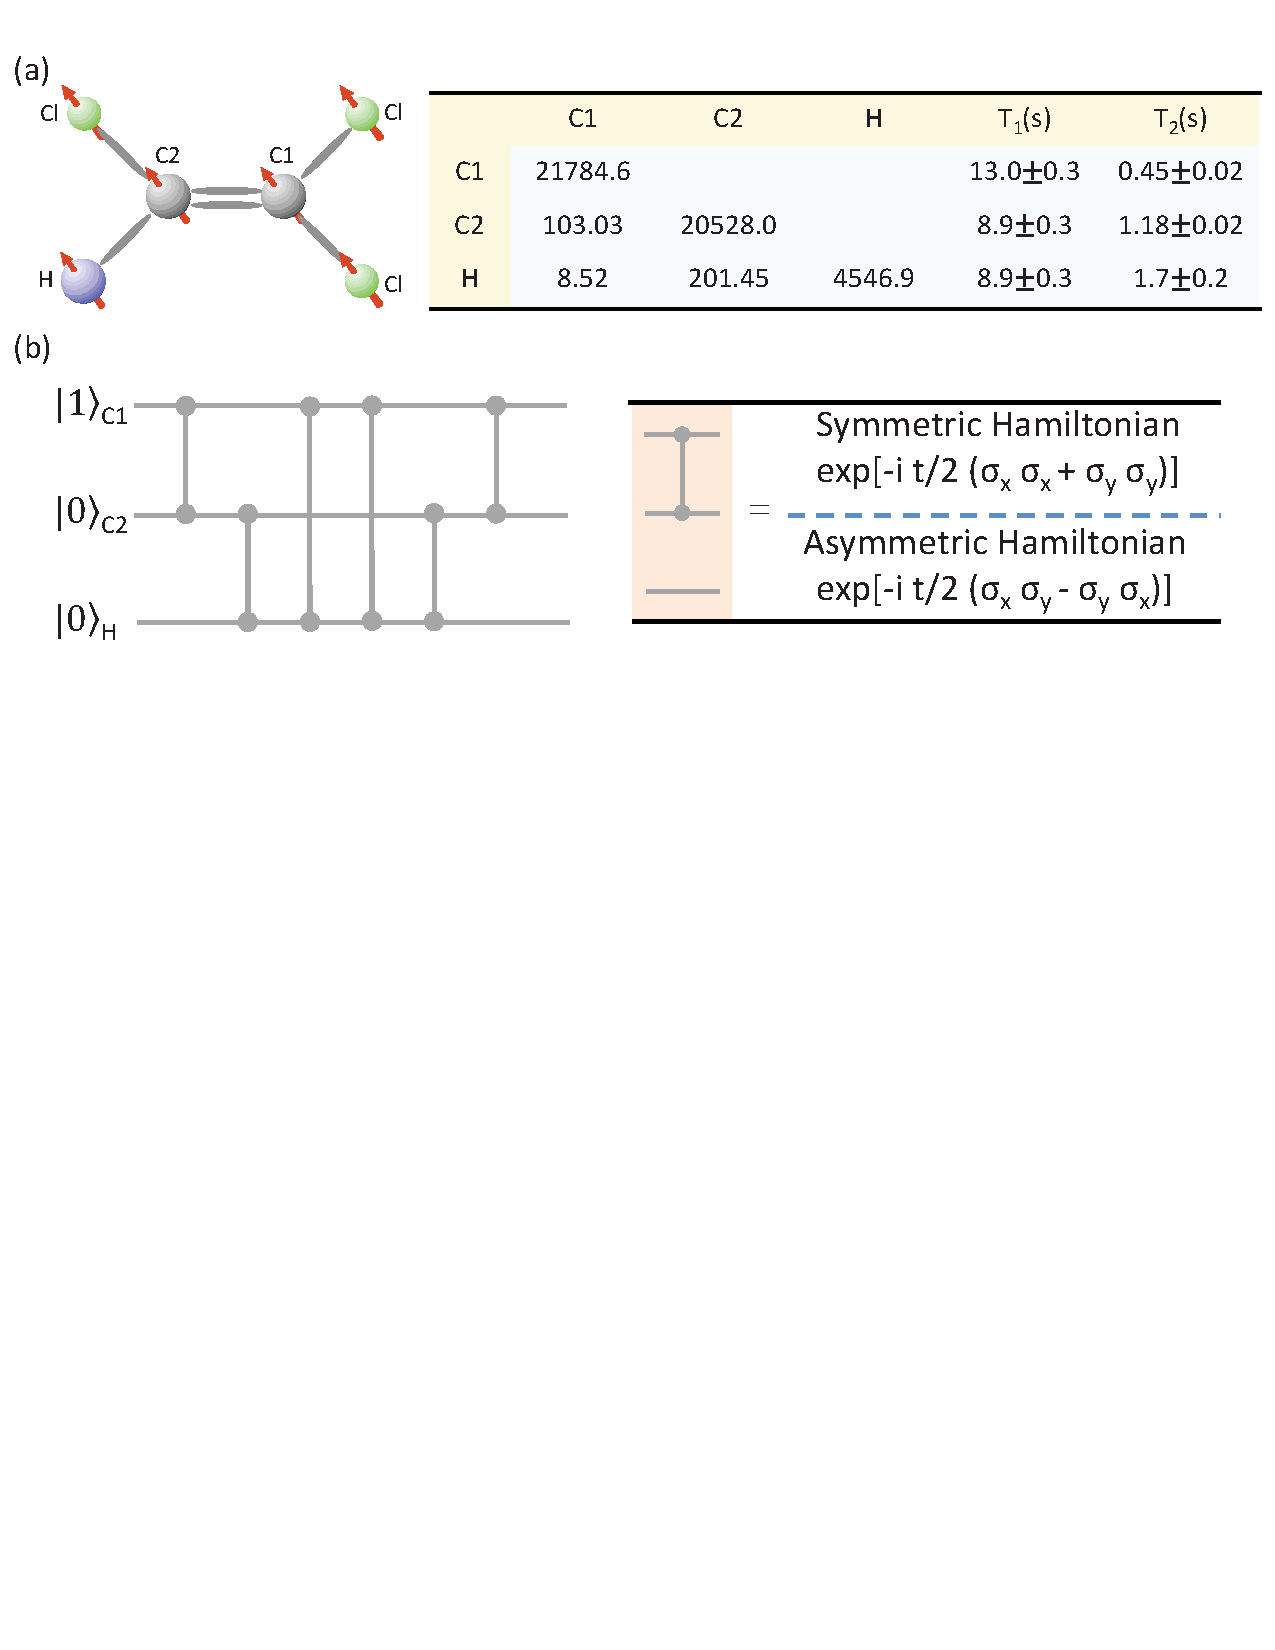
\includegraphics[width=0.9\columnwidth]{molecule.pdf}
\caption{(color online). (a) Experimental implementation of chiral quantum walk in NMR using trichloroethylene in which the two $^{13}$C and one $^{1}$H spins form a 3-qubit sample. In the parameter table  the diagonal elements are the chemical shifts (Hz), and the off-diagonal elements are scalar coupling strengths (Hz).  T$_1$ and T$_2$ are the relaxation and dephasing time scales.  (b) Quantum circuit of implementing chiral quantum walk. The six time evolutions which form a palindromic sequence are dominated by time-symmetric Hamiltonian XX+YY or time-asymmetric Hamiltonian XY-YX}\label{molecule}
\end{figure}

Each experimental procedure consists of three main parts: (A) State Initialization: Preparing the system to the pseudo-pure state (PPS) $\ket{000}$, and then excite one spin to its excitation $\ket{1}$; (B) Evolution: Driving the system evolved under the symmetric or asymmetric Hamiltonian, in a palindromic circuit; (C) Measurement: Measuring the probabilities of finding the excitation in all three spins. Without loss of generality, we will describe the experimental procedure with spin 1 initially excited, $i.e.$,  $\ket{100}$ as the initial state.

(A) State Initialization. Starting from the thermal equilibrium, we first created the pseudo-pure state
\begin{equation}
\rho_{000}=(1-\epsilon)\openone/8+\epsilon \ket{000} \bra{000}
\end{equation}
using the spatial average technique \cite{spatial}. Here $\epsilon \approx 10^{-5}$ qualifies the polarization of the system and $\openone$ is the $8\times 8$ identity matrix. Next, we applied a $\pi$ pulse on spin 1 to rotate it to its excitation $\ket{1}$. This $\pi$ rotation was realized by a  a 2ms and over 99.5\% fidelity GRadient Ascent Pulse Engineering (GRAPE) pulse \cite{grape1,grape2}. Afterwards we achieved the initial state $\ket{100}$.

(B) Evolution. In this part, the initial state $\ket{100}$ will be evolved under four types of Hamiltonians: symmetric Hamiltonian XX+YY and its time reversal, and asymmetric Hamiltonian XY-YX and its time reversal, respectively. The circuit of the whole evolution part is depicted in Fig. \ref{molecule}b, where the six two-body interactions form an palindromic loop for this 3-qubit system. For any interaction with a given time $t$, it can be represented by a unitary operator $e^{-iHt}$, where $H=\pm\frac{1}{2}(\sigma_x\sigma_x+\sigma_y\sigma_y)$ for symmetric case or $H=\pm\frac{1}{2}(\sigma_x\sigma_y-\sigma_y\sigma_x)$ for asymmetric case. In experiment we utilized GRAPE pulses with different lengths to implement all of the two-body interactions, depending on the J-coupling strength (see the table of Fig. \ref{molecule}a) of the related two spins. The three typical lengths of GRAPE pulses for implementing the two-body interactions are 3ms for J$_{12}$, 2ms for J$_{23}$ and 8ms for J$_{13}$, respectively. Therefore, the overall time of the circuit comprised by six evolutions is 26ms, which is not much comparative to the decoherence time. For any Hamiltonian out of the four types, we implemented the circuit for 37 times as $t$ was chosen by every $\pi/18$ step in $[0, 2\pi]$. So the total number of GRAPE pulses in this part is 444, and all of them are guaranteed to be over 99\% fidelity in calculation.

(C) Measurement. After the implementation of the circuit, we measured the probabilities of finding the excitation in all three spins. It means measuring the probabilities of  $\ket{100}$, $\ket{010}$ and $\ket{001}$, which corresponds to traditional population measurements in NMR setup. We used a $\pi/2$ pulse to rotate spin 2 to the transverse $x-y$ plane and compared the intensity of the relative transition with the initial state. Then all the three probabilities could be obtained.

\section{Experimental Results}

\begin{figure}[h] \centering
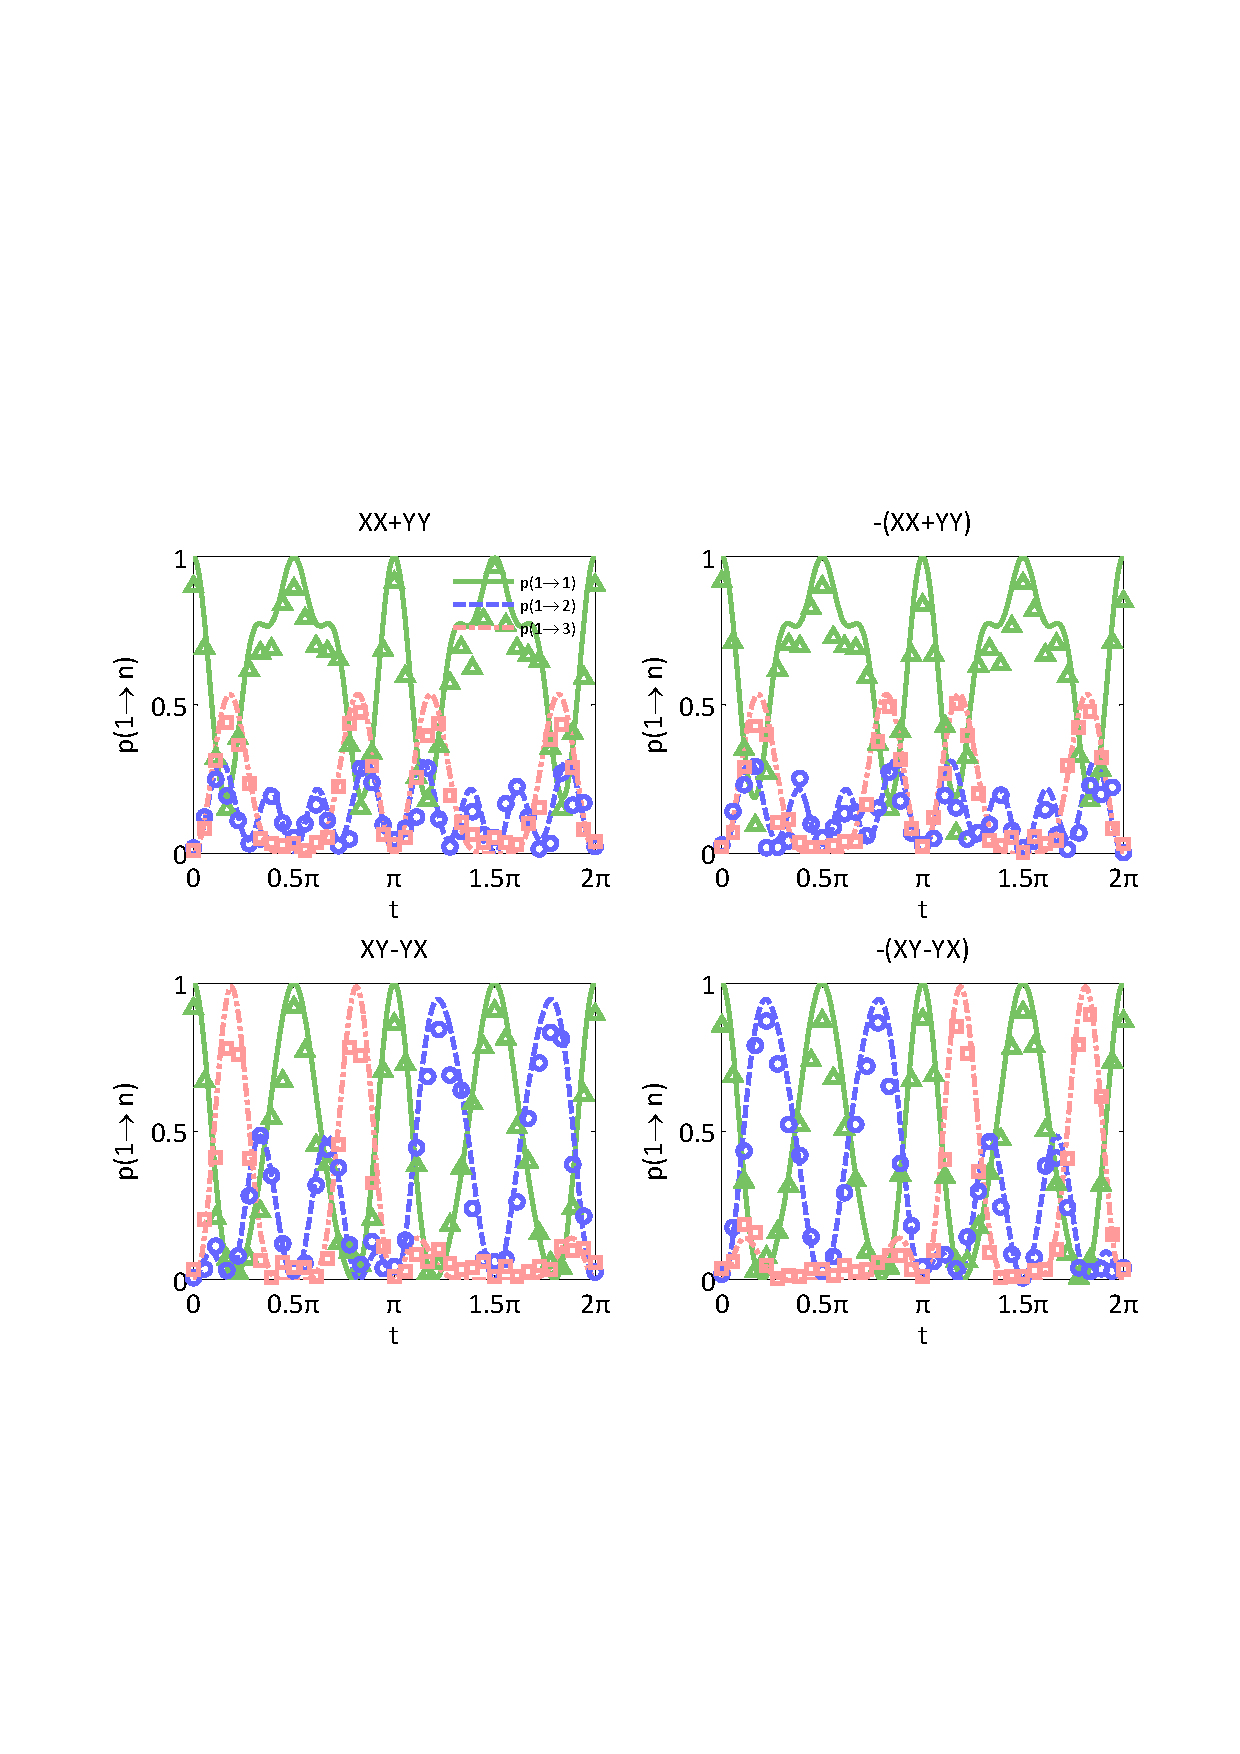
\includegraphics[width=0.9\columnwidth]{exp_1.pdf}
\caption{(color online). (a) Experimental results of implementing the chiral quantum walk the 3-qubit NMR system. The initial state $\ket{100}$ is represented by an excitation on spin 1. The green, blue and red curves are the theoretical probabilities of finding $\ket{100}$, $\ket{010}$ and $\ket{001}$, while the triangles, circuits and squares are the related experimental results. All probabilities are measured every $\pi/18$ time in experiment. The two plots in the top correspond to the time-symmetric Hamiltonian and its time-reversed evolution, which cannot break the time symmetry. The two plots in the bottom correspond to the time-asymmetric Hamiltonian and its time-reversed evolution, which do break the time symmetry.}\label{exp_1}
\end{figure}

In this section we still take the initial excitation state $\ket{100}$ as the example. Our theory predicts that for the time-symmetric Hamiltonian XX+YY, we cannot break the time symmetry because of the palindromic circuit in Fig. \ref{molecule}b, nor enhance the transport probabilities. The experimental data depicted in the two plots on the top of Fig. \ref{exp_1} illustrate a well-matched result with the theoretical prediction. The green, blue and red curves are the theoretical probabilities of finding $\ket{100}$, $\ket{010}$ and $\ket{001}$, respectively. The triangles, circuits and squares show the experimental results of the aforementioned probabilities. We can clearly see in the top left panel the probabilities of finding the excitation in spin 2 or spin 3 are always bounded to a certain value below 0.6, which means the quantum transport process is suppressed. In the top right panel since the time symmetry cannot be broken under the time-symmetric Hamiltonian, we obtained almost the same plot as the left one.

The theory also tells by applying the gates that break time symmetry in the same palindromic sequence can break the time symmetry, as well as generating a large enhancement of the transport rates of the excitation. In experiment the time-asymmetric Hamiltonian was used to achieve this time symmetry breaking. On the bottom of Fig. \ref{exp_1}, we see that the probabilities of encountering the excitation in spin 2 or spin 3 can reach almost one, not only from the theory but also from the experiment. It demonstrates the enhancement of the quantum transport of the excitation. Moreover, in the right bottom panel we can see the time symmetry is broken by applying the time-reversed evolution.

\begin{figure}[h] \centering
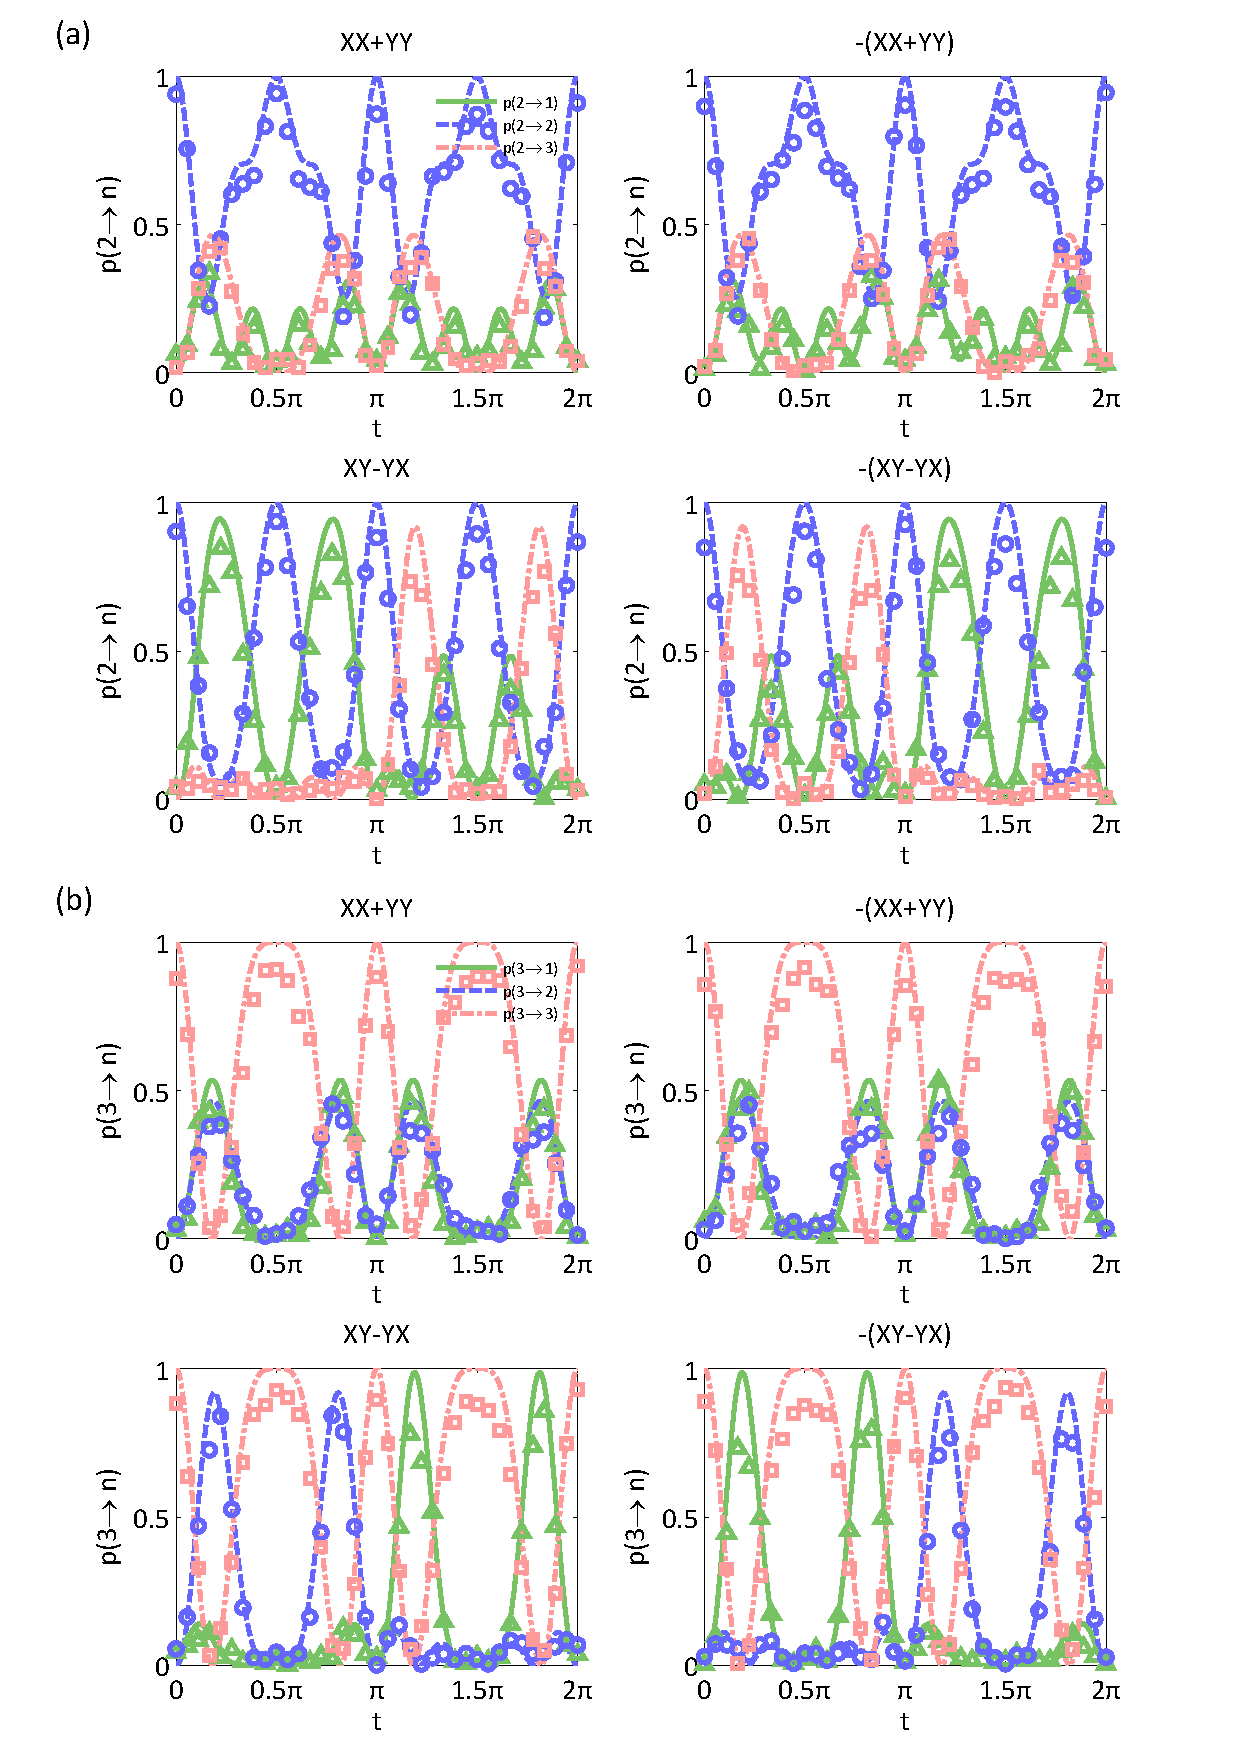
\includegraphics[width=0.9\columnwidth]{exp_23.pdf}
\caption{(color online). (a) Experimental results with the initial excitation state $\ket{010}$. (b) Experimental results with the initial excitation state $\ket{001}$.}\label{exp_23}
\end{figure}

Besides the experiments with the initial excitation being on spin 1, we also investigated the other two cases that the initial excitation states localized on $\ket{010}$ and $\ket{001}$. The experimental results are displayed in Fig.  \ref{exp_23}, which show similar properties of time symmetric breaking and suppression or enhancement of transport probabilities.

The difference between theory and experiment can be attributed to two factors: the imperfection of the GRAPE pulses, as in each circuit six 99\% fidelity GRAPE pulses are used, which may accumulate some unexpected errors; the decoherence issues, as 26ms of total evolution time may induce a certain amount of signal loss due to spin decoherence. 

\begin{thebibliography}{35}
\expandafter\ifx\csname natexlab\endcsname\relax\def\natexlab#1{#1}\fi
\expandafter\ifx\csname bibnamefont\endcsname\relax
  \def\bibnamefont#1{#1}\fi
\expandafter\ifx\csname bibfnamefont\endcsname\relax
  \def\bibfnamefont#1{#1}\fi
\expandafter\ifx\csname citenamefont\endcsname\relax
  \def\citenamefont#1{#1}\fi
\expandafter\ifx\csname url\endcsname\relax
  \def\url#1{\texttt{#1}}\fi
\expandafter\ifx\csname urlprefix\endcsname\relax\def\urlprefix{URL }\fi
\providecommand{\bibinfo}[2]{#2}
\providecommand{\eprint}[2][]{\url{#2}}


\bibitem[{\citenamefont{Vandersypen and Chuang}(2005)}]{nmrreview}
\bibinfo{author}{\bibfnamefont{L.~M.} \bibnamefont{Vandersypen}}
  \bibnamefont{and} \bibinfo{author}{\bibfnamefont{I.~L.}
  \bibnamefont{Chuang}}, \bibinfo{journal}{Reviews of Modern Physics}
  \textbf{\bibinfo{volume}{76}}, \bibinfo{pages}{1037} (\bibinfo{year}{2005}),
  \urlprefix\url{http://rmp.aps.org/abstract/RMP/v76/i4/p1037_1}.

\bibitem[{\citenamefont{Cory et~al.}(1997)\citenamefont{Cory, Fahmy, and
  Havel}}]{spatial}
\bibinfo{author}{\bibfnamefont{D.~G.} \bibnamefont{Cory}},
  \bibinfo{author}{\bibfnamefont{A.~F.} \bibnamefont{Fahmy}}, \bibnamefont{and}
  \bibinfo{author}{\bibfnamefont{T.~F.} \bibnamefont{Havel}},
  \bibinfo{journal}{Proceedings of the National Academy of Sciences}
  \textbf{\bibinfo{volume}{94}}, \bibinfo{pages}{1634} (\bibinfo{year}{1997}),
  \urlprefix\url{http://www.pnas.org/content/94/5/1634.short}.

\bibitem[{\citenamefont{Khaneja et~al.}(2005)\citenamefont{Khaneja, Reiss,
  Kehlet, Schulte-Herbr{\"u}ggen, and Glaser}}]{grape1}
\bibinfo{author}{\bibfnamefont{N.}~\bibnamefont{Khaneja}},
  \bibinfo{author}{\bibfnamefont{T.}~\bibnamefont{Reiss}},
  \bibinfo{author}{\bibfnamefont{C.}~\bibnamefont{Kehlet}},
  \bibinfo{author}{\bibfnamefont{T.}~\bibnamefont{Schulte-Herbr{\"u}ggen}},
  \bibnamefont{and} \bibinfo{author}{\bibfnamefont{S.~J.}
  \bibnamefont{Glaser}}, \bibinfo{journal}{Journal of Magnetic Resonance}
  \textbf{\bibinfo{volume}{172}}, \bibinfo{pages}{296} (\bibinfo{year}{2005}),
  \urlprefix\url{http://www.sciencedirect.com/science/article/pii/S1090780704003696}.

\bibitem[{\citenamefont{Ryan et~al.}(2008)\citenamefont{Ryan, Negrevergne,
  Laforest, Knill, and Laflamme}}]{grape2}
\bibinfo{author}{\bibfnamefont{C.}~\bibnamefont{Ryan}},
  \bibinfo{author}{\bibfnamefont{C.}~\bibnamefont{Negrevergne}},
  \bibinfo{author}{\bibfnamefont{M.}~\bibnamefont{Laforest}},
  \bibinfo{author}{\bibfnamefont{E.}~\bibnamefont{Knill}}, \bibnamefont{and}
  \bibinfo{author}{\bibfnamefont{R.}~\bibnamefont{Laflamme}},
  \bibinfo{journal}{Physical Review A} \textbf{\bibinfo{volume}{78}},
  \bibinfo{pages}{012328} (\bibinfo{year}{2008}),
  \urlprefix\url{http://pra.aps.org/abstract/PRA/v78/i1/e012328}.

\end{thebibliography}
\end{document}


